\documentclass[9pt,aspectratio=169]{beamer}

\usetheme{Warsaw}

\usepackage{fancyvrb}
\usepackage{lmodern}
\usepackage[sfdefault,light,lining]{FiraSans}
\usepackage{listings}
\usepackage{xcolor}
\usepackage{tikz}
\usetikzlibrary{positioning,arrows.meta,shapes.geometric}
\usepackage{booktabs}
\usepackage{array}
\usepackage{graphicx}

\definecolor{LogicBlue}{RGB}{204,0,0}
\definecolor{InferenceRed}{RGB}{212,55,59}
\definecolor{linkblue}{HTML}{0066FF}
\definecolor{LiteRed}{RGB}{248,232,232}

\setbeamercolor{structure}{fg=InferenceRed}
\setbeamercolor{frametitle}{bg=LogicBlue,fg=white}
\setbeamercolor{palette primary}{bg=LogicBlue,fg=white}
\setbeamercolor{palette secondary}{bg=InferenceRed,fg=white}
\setbeamercolor{block title}{bg=LogicBlue,fg=white}
\setbeamercolor{block body}{bg=LiteRed,fg=black}

\setbeamertemplate{headline}{\vspace{0.4cm}}
\setbeamertemplate{section in head/foot}{}
\setbeamertemplate{subsection in head/foot}{}
\setbeamertemplate{mini frames}{}
\setbeamertemplate{navigation symbols}{}

\setbeamertemplate{footline}{
  \hfill
  \usebeamercolor[fg]{page number in head/foot}
  \usebeamerfont{page number in head/foot}
  \insertframenumber\,/\,\inserttotalframenumber\kern1em
  \vbox{\vskip0pt}
}
\setbeamercolor{page number in head/foot}{fg=black}

\setbeamersize{text margin left=0.45cm, text margin right=0.45cm}
\hypersetup{colorlinks=true,urlcolor=linkblue}

\lstset{
  basicstyle=\ttfamily\scriptsize,
  keywordstyle=\bfseries,
  commentstyle=\itshape\color{gray},
  breaklines=true,
  frame=single,
  backgroundcolor=\color{black!4},
  xleftmargin=2pt, xrightmargin=2pt,
  columns=fullflexible,
  keepspaces=true,
  showstringspaces=false
}

\newcommand{\screenslide}[1]{%
\begin{frame}[plain]
  \vspace*{0.10cm}
  \centering
  \includegraphics[width=\paperwidth,height=0.92\paperheight,keepaspectratio]{#1}
\end{frame}}

\title{How to Design Agentic Systems?}
\subtitle{Hybrid Agentic Workflows for Software Analytics}
\author{Tim Menzies}
\institute{prof, cs, \textbf{ncstate}, usa\\
  acm-ieee-ase fellow; eic ASEj\\
  timm@ieee.org\newline\url{http://timm.fyi}}
\date{Mar 13, 2025}
\begin{document}

\begin{frame}
\titlepage
\end{frame}

\begin{frame}{Motivation: The ``just throw an LLM at it'' phase is ending}
\textbf{Claim:} agentic software will stay; pure-LLM monocultures will not.

\vspace{3mm}
\footnotesize
The engineering question is not ``can an LLM do it?'' but ``which parts should remain typed, searchable, and cheap?''


\vspace{3mm}
\begin{itemize}
\item Pure-LLM systems are expensive, variable, and hard to reproduce.
\item Real software analytics needs \textbf{repeatability}, \textbf{traceability}, and \textbf{cheap search}.
\item The survivors will be \textbf{hybrids}: symbolic checks, classic learners, search-based optimization, RL, and only \emph{targeted} LLM components.
\end{itemize}

\end{frame}


\screenslide{beamer_assets/agentic.png}
\screenslide{beamer_assets/problems.png}
\screenslide{beamer_assets/better.png}

\begin{frame}{<u Unfair Advantage: 30 Years of Mining Work}
\begin{itemize}
\item Three decades of SE analytics means we are \textbf{not starting from zero}.
\item 300+ papers give us a mineable corpus of constraints, defaults, caveats, and proven mitigations.
\item Earlier work already solved hard parts of the search problem:\newline
      SPL configuration, SBSE, hyperparameter optimization, compact AI, and large feature spaces.
\item I now also have \textbf{new stochastic probes} that reveal the internal landscape of these optimization problems and give dramatic shortcuts through the search.
\end{itemize}

\vspace{3mm}
\begin{block}{Not a green-field project}
This is decades of verified tricks plus a newer understanding of the optimization landscape.
\end{block}
\end{frame}

\begin{frame}{Class Hierarchy: LLM and Non-LLM as Siblings}
\centering
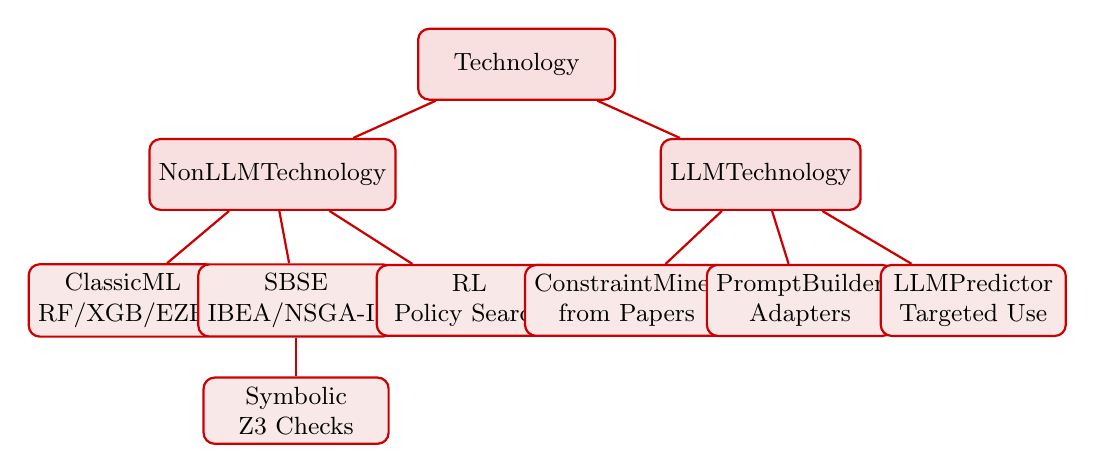
\begin{tikzpicture}[
  every node/.style={font=\small, align=center},
  box/.style={draw=LogicBlue, rounded corners, thick, fill=LiteRed, minimum width=2.35cm, minimum height=0.82cm},
  topbox/.style={draw=LogicBlue, rounded corners, thick, fill=LogicBlue!12, minimum width=2.5cm, minimum height=0.9cm},
  line/.style={draw=LogicBlue, thick}
]
\node[topbox] (tech) at (0,2.2) {Technology};
\node[topbox] (nollm) at (-3.1,0.8) {NonLLMTechnology};
\node[topbox] (llm) at (3.1,0.8) {LLMTechnology};

\node[box] (ml) at (-5.0,-0.8) {ClassicML\\RF/XGB/EZR};
\node[box] (sbse) at (-2.8,-0.8) {SBSE\\IBEA/NSGA-II};
\node[box] (rl) at (-0.6,-0.8) {RL\\Policy Search};
\node[box] (z3) at (-2.8,-2.2) {Symbolic\\Z3 Checks};

\node[box] (miner) at (1.4,-0.8) {ConstraintMiner\\from Papers};
\node[box] (prompt) at (3.6,-0.8) {PromptBuilder\\Adapters};
\node[box] (pred) at (5.8,-0.8) {LLMPredictor\\Targeted Use};

\draw[line] (tech) -- (nollm);
\draw[line] (tech) -- (llm);
\draw[line] (nollm) -- (ml);
\draw[line] (nollm) -- (sbse);
\draw[line] (nollm) -- (rl);
\draw[line] (sbse) -- (z3);
\draw[line] (llm) -- (miner);
\draw[line] (llm) -- (prompt);
\draw[line] (llm) -- (pred);
\end{tikzpicture}

\vspace{2mm}
\small
LLM components are not the whole system. They are one subclass inside a larger typed ecosystem.
\end{frame}

\screenslide{beamer_assets/10.png}
\screenslide{beamer_assets/11.png}
\screenslide{beamer_assets/12.png}
\screenslide{beamer_assets/13.png}
\screenslide{beamer_assets/14.png}
\screenslide{beamer_assets/15.png}
\screenslide{beamer_assets/17.png}
\screenslide{beamer_assets/18.png}
\screenslide{beamer_assets/19.png}

\screenslide{beamer_assets/rolling.png}

\begin{frame}[fragile]{Type-Safe Polymorphic Agents}
\begin{lstlisting}[language=Python]
from abc import ABC, abstractmethod
from dataclasses import dataclass

@dataclass
class Prediction:
    value: object
    why: str

class Agent(ABC):
    @abstractmethod
    def predict(self, x) -> Prediction: ...

class ClassicRF(Agent):     # in: Vector
    def predict(self, x: Vector) -> Prediction: ...

class EZR(Agent):           # in: Table
    def predict(self, x: Table) -> Prediction: ...

class LLMPredictor(Agent):  # in: CodeString
    def predict(self, x: CodeString) -> Prediction: ...

class GAOptimizer(Agent):   # in: Population
    def predict(self, x: Population) -> Prediction: ...
\end{lstlisting}

\small One interface, many paradigms. The orchestrator asks: what type goes in, what type comes out, and what checks are required?
\end{frame}

\begin{frame}[fragile]{Experience $\rightarrow$ Small Fixes in the Same Language}
\begin{columns}[T]
\begin{column}{0.54\textwidth}
\begin{lstlisting}
# config.yaml (mined from papers)
pipeline:
  preprocessor:        # XOR
    - CodeEmbedder:
        out: Vector
    - TextPromptBuilder:
        out: CodeString
  learner:             # XOR
    - ClassicRF:    {in: Vector}
    - EZR:          {in: Table}
    - LLMPredictor: {in: CodeString}
    - GAOptimizer:  {in: Population}

constraints:
  - if: LLMPredictor
    require: StabilityCheck
  - if: ClassicRF
    require: TenFoldCrossVal
\end{lstlisting}
\end{column}
\begin{column}{0.42\textwidth}
\small
\textbf{Key design trick:}

\medskip
``Experience shows X is a problem''
$\rightarrow$ add one new node in the same tree.

\medskip
\begin{itemize}
\item LLMs vary? add \texttt{StabilityCheck}
\item learners overfit? add \texttt{TenFoldCrossVal}
\item search explodes? add \texttt{LandscapeProbe}
\end{itemize}

\medskip
So problems become \textbf{small composable additions}, not architectural rewrites.
\end{column}
\end{columns}
\end{frame}

\begin{frame}[fragile]{The ``Why Engine'': Solver-Backed Rejection}
\begin{columns}[T]
\begin{column}{0.54\textwidth}
\begin{lstlisting}[language=Python]
from z3 import *

LLM   = Bool('LLMPredictor')
Stab  = Bool('StabilityCheck')
CV    = Bool('TenFoldCrossVal')
RF    = Bool('ClassicRF')

s = Solver()
s.add(Implies(LLM, Stab))
s.add(Implies(RF, CV))

s.push()
s.add(LLM == True, Stab == False)

if s.check() == unsat:
    print("REJECTED")
    print(rationale["LLM->Stab"])
\end{lstlisting}
\end{column}
\begin{column}{0.42\textwidth}
\small
\textbf{Runtime story:}
\begin{enumerate}
\item propose a candidate pipeline
\item check structure, types, and risk rules
\item \textbf{SAT} $\rightarrow$ run it
\item \textbf{UNSAT} $\rightarrow$ reject instantly
\item explain \emph{why} in human language
\end{enumerate}

\medskip
Old lab experience becomes live tutoring, not tribal memory.
\end{column}
\end{columns}
\end{frame}

\begin{frame}{Architecture: A Hybrid Agentic Loop}
\centering
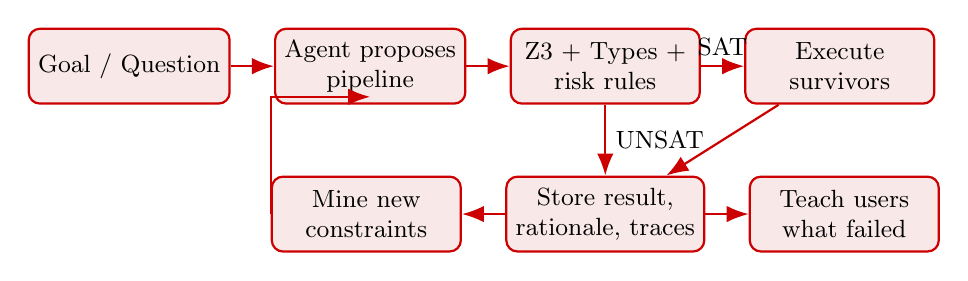
\begin{tikzpicture}[
  node distance=0.9cm and 0.55cm,
  every node/.style={font=\small, align=center},
  box/.style={draw=LogicBlue, rounded corners, thick, fill=LiteRed, minimum width=2.4cm, minimum height=0.95cm},
  arr/.style={-{Latex[length=2.8mm]}, thick, draw=LogicBlue}
]
\node[box] (goal) {Goal / Question};
\node[box, right=of goal] (propose) {Agent proposes\\pipeline};
\node[box, right=of propose] (check) {Z3 + Types +\\risk rules};
\node[box, right=of check] (run) {Execute\\survivors};
\node[box, below=of check] (learn) {Store result,\\rationale, traces};
\node[box, left=of learn] (mine) {Mine new\\constraints};
\node[box, right=of learn] (teach) {Teach users\\what failed};

\draw[arr] (goal) -- (propose);
\draw[arr] (propose) -- (check);
\draw[arr] (check) -- node[above]{SAT} (run);
\draw[arr] (check) -- node[right]{UNSAT} (learn);
\draw[arr] (run) -- (learn);
\draw[arr] (learn) -- (mine);
\draw[arr] (learn) -- (teach);
\draw[arr] (mine.west) |- ([yshift=0.10cm]propose.south);
\end{tikzpicture}

\vspace{3mm}
\small
Agentic---but not reckless. Search is allowed; unsafe combinations are not.
\end{frame}

\begin{frame}{Roadmap}
\begin{enumerate}
\item Mine the corpus into constraints, objectives, and caveats.
\item Annotate components with explicit input/output types.
\item Build the class hierarchy and adapter layer for LLM and non-LLM components.
\item Wire Z3 to reject bad combinations before execution.
\item Use stochastic probes to shrink the search landscape.
\item Run agentic orchestration only on safe, typed survivors.
\item Capture rationales so the system explains itself to users and students.
\end{enumerate}
\end{frame}

\begin{frame}{Why Me, Why Now}
\begin{itemize}
\item I have the archive: three decades of mined SE analytics results.
\item I have the old machinery: SBSE, feature models, compact learners, and optimizer experience.
\item I have the new angle: stochastic methods that expose the inner landscape and shorten the search.
\item I have the teaching use-case: a system that trains the next generation while doing real work.
\end{itemize}

\vspace{4mm}
\begin{block}{Closing pitch}
This is exactly the moment to connect LLM mining with non-LLM optimization and symbolic safety.
\end{block}
\end{frame}

\end{document}
